\label{sec:xadd}

We begin with a formal definition of the extended algebraic decision
diagram (XADD), then in Section~\ref{sec:approx} we will contribute
approximation techniques for XADDs and in Section~\ref{sec:basdp}, we
will show how this approximation can be used in a bounded
approximate symbolic dynamic programming algorithm for hybrid MDPs.

\subsection{Case Semantics of XADDs}

%% THIS PAPER DOES NOT ALLOW POLYNOMIALS, SHOULD NOT MENTION THEM!

%% Need to make strong immediate connections between cases and
%% XADDs since XADDs have already been introduced and discuss why
%% you're taking the time to discuss the case representation.

Underlying the XADD of Figure~\ref{fig:stepfunfig} is a simple
piecewise linear function that we can represent in mathematical case
form that we use as a semantical representation of XADDs throughout
this paper.  Specifically, given a domain of boolean and continuous
variables $(\vec{b},\vec{x}) = ( b_1,\ldots,b_n,x_{1},\ldots,x_m )$,
where $b_i \in \{ 0,1 \}$ ($1 \leq i \leq n$) and $x_j \in
[x_j^{\min},x_j^{\max}]$ ($1 \leq j \leq m$) for
$x_j^{\min},x_j^{\max} \in \mathbb{R}$ and $x_j^{\max} > x_j^{\min}$, a case
statement with linear piece constraints and linear values has the form
{\footnotesize 
\begin{align}
f(\vec{b},\vec{x}) = 
\begin{cases}
  \phi_1(\vec{b},\vec{x}): & f_1(\vec{x}) \\ 
 \vdots&\vdots\\ 
  \phi_k(\vec{b},\vec{x}): & f_k(\vec{x}) \\ 
\end{cases} \, . \label{eq:case}
\end{align}
} 
%% The XADD could work with a full set of inequalities, it's not
%% worth discussing complications of only $<,>$ at this point in
%% the paper.  You want to get to Section 3 -- the contribution --
%% as soon as possible.
%%
%% The partial function details of XADDs do not play any role in
%% this paper, they only occur in the SDP backup and were covered
%% in previous work -- its irrelevant here.
Here the $f_i$ are linear expressions over $\vec{x}$ and the $\phi_i$
are logical formulae defined over the domain $(\vec{b},\vec{x})$ that
can include arbitrary logical ($\land,\lor,\neg$) combinations of (i)
boolean variables and (ii) linear inequalities over $\vec{x}$.

In the XADD examples of Figure~\ref{fig:stepfunfig}, we note that 
\emph{every leaf} represents a case value $f_i$ and 
\emph{every path from root to leaf} represents a conjunction
of decision constraints.  The disjunction of all path constraints
leading to leaf $f_i$ corresponds to a case partition
$\l \phi_i(\vec{b},\vec{x}) : f_i(\vec{x}) \r$.  Clearly, all case
partitions derived from an XADD must be mutually disjoint and
exhaustive of the domain $(\vec{b},\vec{x})$ and hence the 
case statement for a XADD $f(\vec{b},\vec{x})$ must be a well-defined
function.

%% This is not important for XADD approximation... it has been
%% covered in previous work for SDP that is cited.
%
%The $\phi_i$ are required to be mutually disjoint from each other;
%however they may not exhaustively cover the state space, in which case
%$f$ is a \emph{partial function}, undefined for some variable
%assignments. Since they represent parts of the piecewise function,
%pairs $(f_i,\phi_i)$ are referred to as cases or partitions of $f$,
%moreover, these are identified with a piecewise function of a single
%partition, which is called a case function.

%% Because we only work with linear XADDs, make this restriction up
%% front as I've done above... then this entire paragraph collapses
%% to a short discussion of the polytopes.
%%
%% Theta is a really bad choice for polytopes since it almost always
%% entails a parameter vector in the AI literature.
%
%We are especially interested in piecewise linear functions and case
%linear functions, in which case all $f_i$ and all expressions in the
%inequalities in $\phi_i$ are linear. 
Since $\phi_i$ can be written in disjunctive normal form (DNF), i.e.,
$\phi_i \equiv \bigvee_{j=0}^{n_i} \theta_{ij}$ where $\theta_{ij}$
represents a conjunction of linear constraints over $\vec{x}$ and a
(partial) truth assignment to $\vec{b}$, we observe that every
$\theta_{ij}$ contains a bounded convex linear polytope ($\vec{x}$ is
finitely bounded in all dimensions as initially defined).  Since this
polytope intepretation will become important for XADD approximation,
we formally define the union of all convex linear polytopes contained in 
$\phi_i$ as
%\begin{equation*}
$C(\phi_i) = \bigcup_j \PT(\theta_{ij})$, 
%\end{equation*}
where $\PT$ extracts the subset of linear constraints from
$\theta_{ij}$. Figure~\ref{fig:symbex} illustrates the defined concepts for an example function.

\vspace{-5mm}
\begin{figure}[ht!]
\begin{minipage}{0.15\textwidth}
{\scriptsize
\begin{align*}
f(x,y)= 
\begin{cases}
  \phi_1:& \hspace{-2mm} f_1\\ 
  \phi_2: & \hspace{-2mm}f_2\\ 
\end{cases}
\end{align*} }
\end{minipage}
\begin{minipage}{0.15\textwidth}
{\scriptsize
\begin{align*}
 \phi_1 = \theta_{11}\vee \theta_{12}\\
\theta_{11} = x<0 \\
\theta_{12} = x>0 \wedge y<0 \\
 f_1 = \displaystyle \frac{x}{2} 
\end{align*} }
\end{minipage}
\begin{minipage}{0.15\textwidth}
{\scriptsize
\begin{align*}
\phi_2 = \theta_{21}\\
\theta_{21} = x>0 \wedge y>0\\
f_2 = \displaystyle -\frac{x}{2}
\end{align*} }
\end{minipage}\\
\begin{minipage}{0.3\textwidth}
\center
\vspace{-13mm}
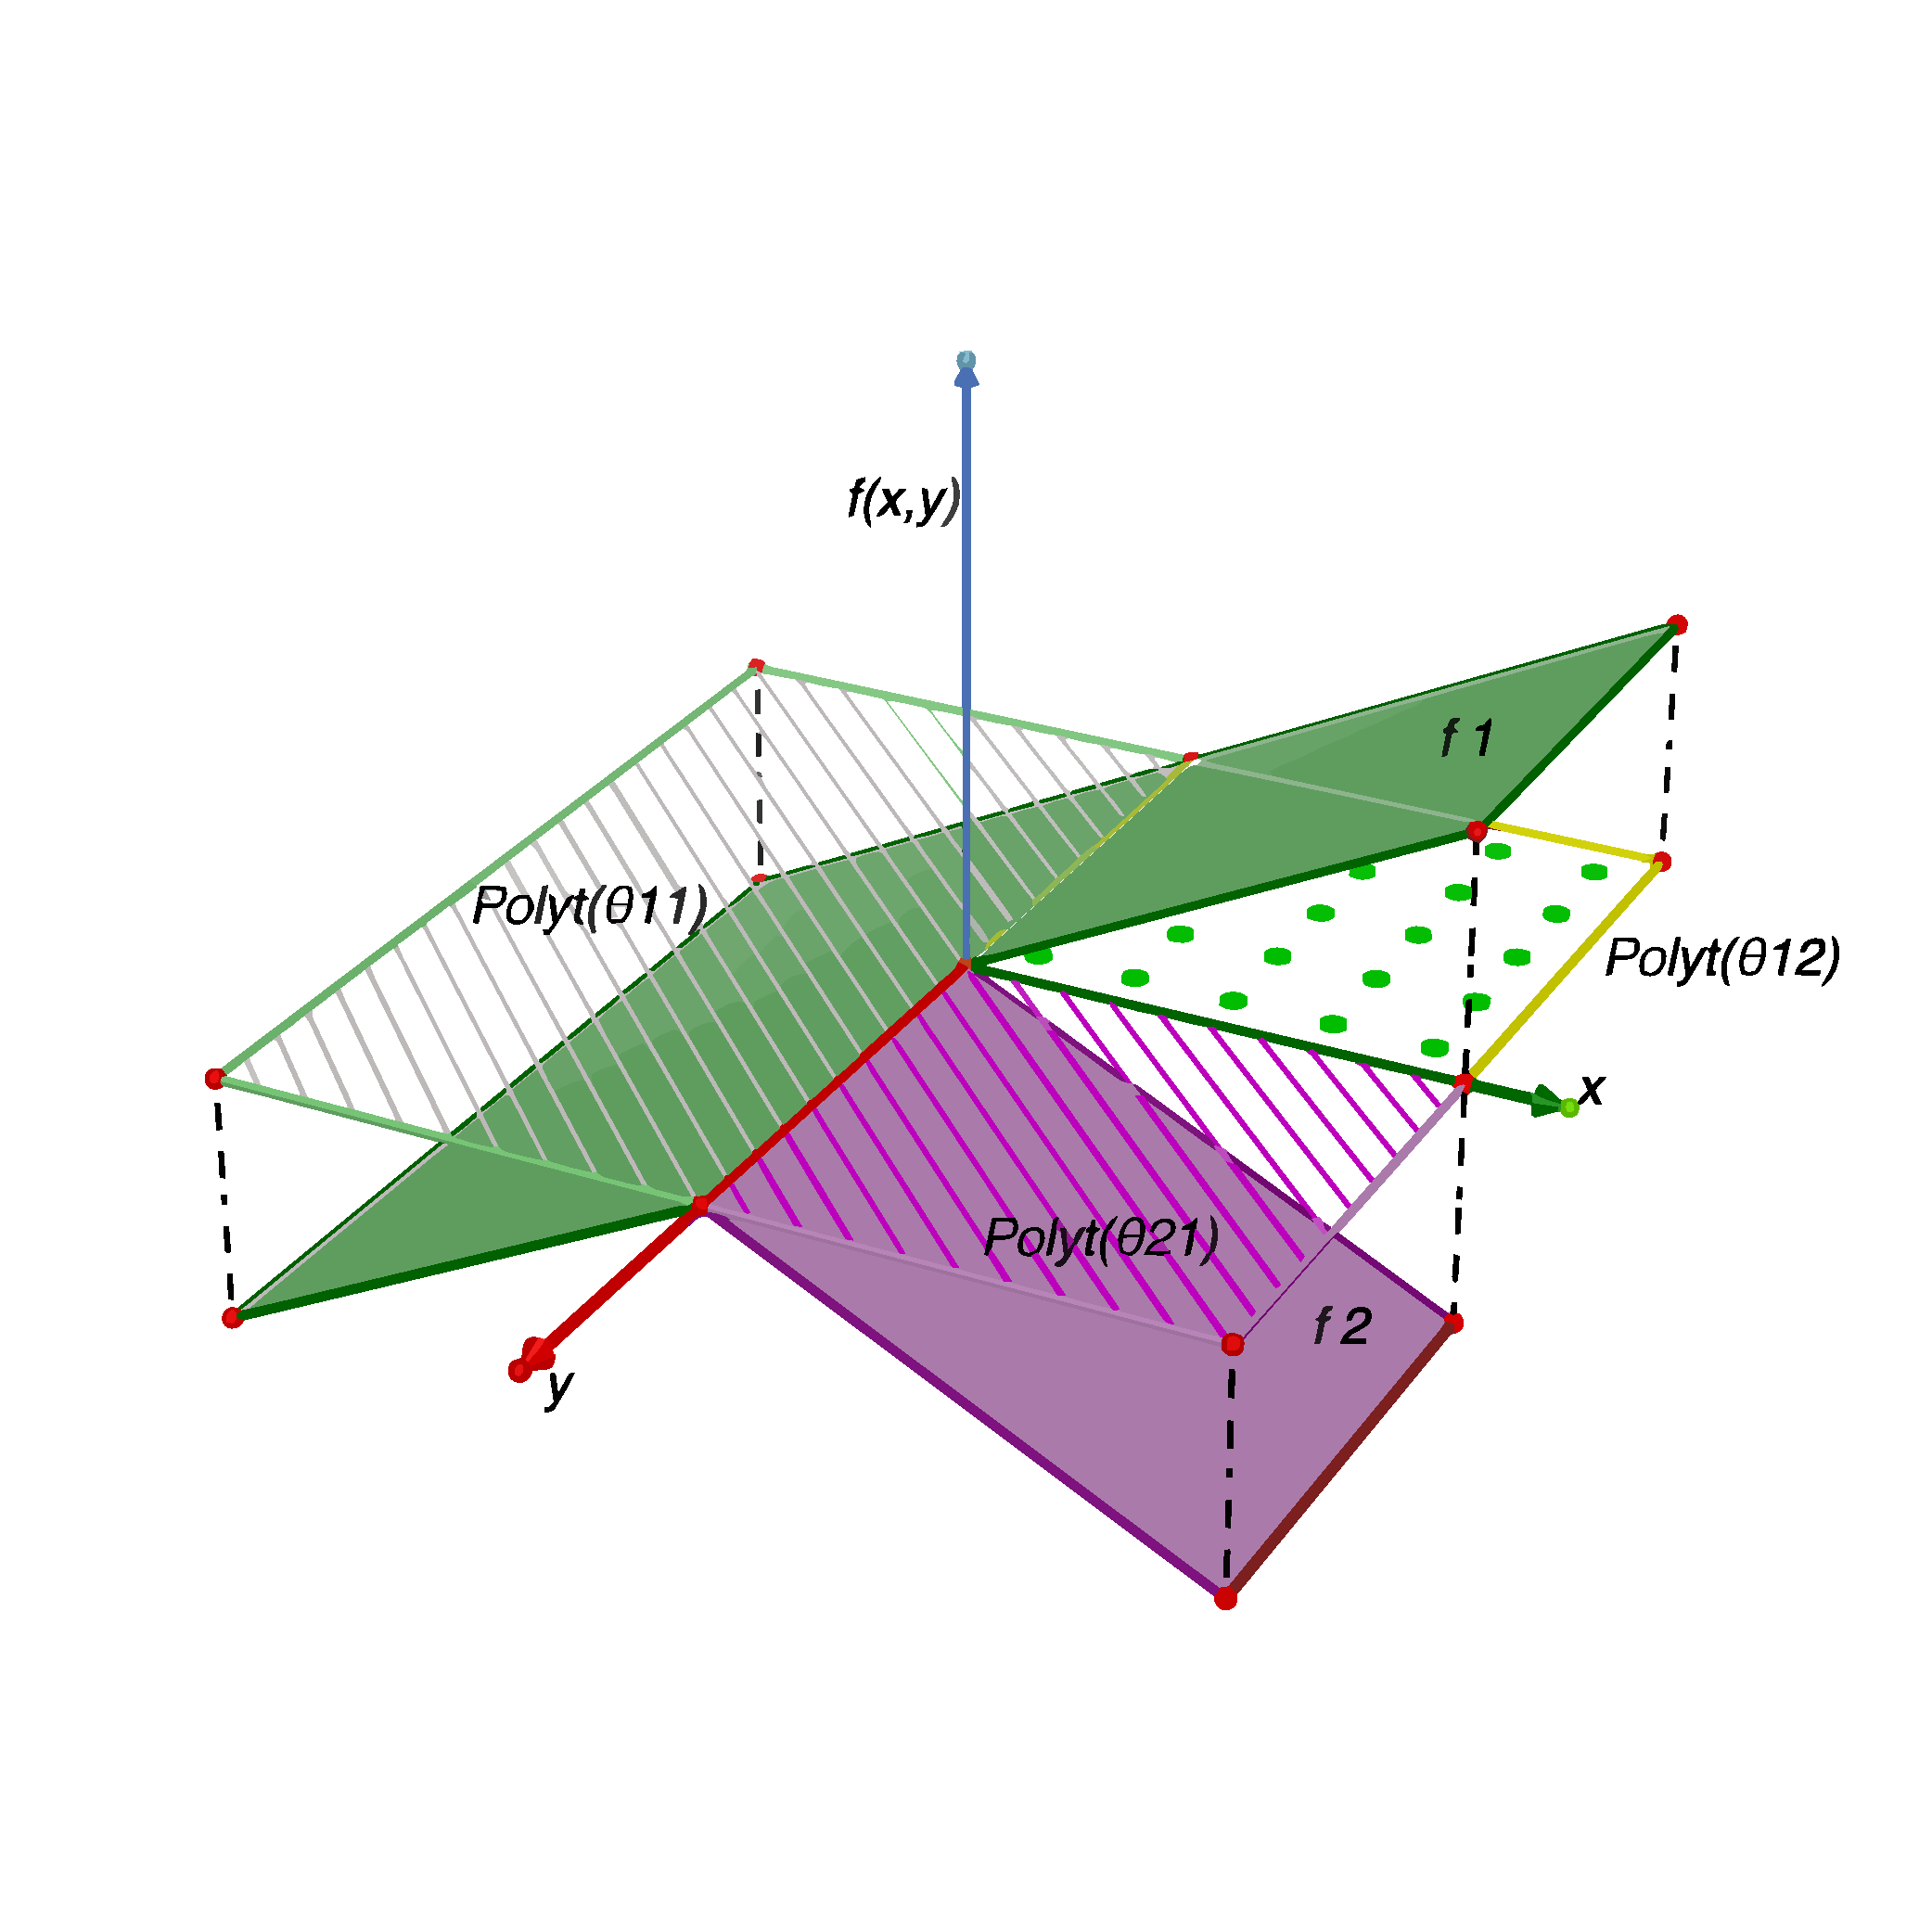
\includegraphics[trim = 1cm 0cm 1cm 0cm,width=\textwidth]{Figures/stepfun/PiecewiseLinearEx.pdf} 
\end{minipage}
\begin{minipage}{0.15\textwidth}
\center
\vspace{-13mm}
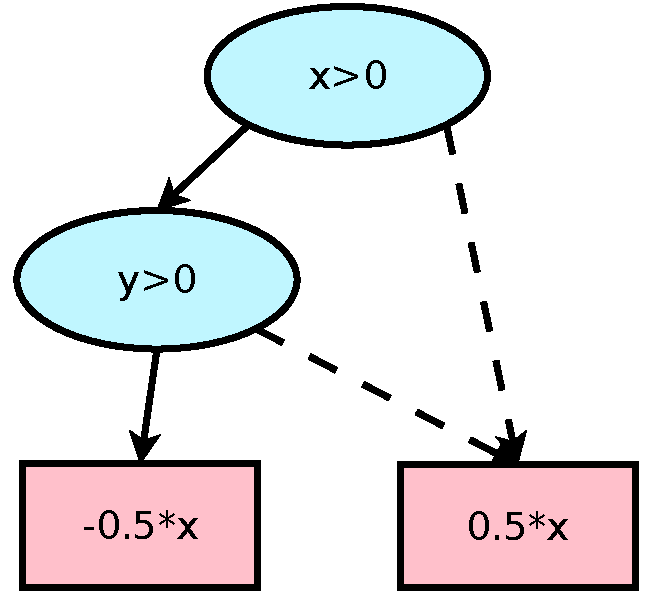
\includegraphics[width=\textwidth]{Figures/xadds/dia2.pdf}
\end{minipage}
\vspace{-10mm}

\caption{Example of piecewise linear function in case and XADD form: \emph{(top)} Case formulation; \emph{(left)} Graphical plot; and \emph{(right)} XADD diagram.}
\label{fig:symbex}
\end{figure}

\subsection{XADD Operations} 

XADDs are important not only because they compactly represent piecewise
functions that arise in the forthcoming solution of hybrid MDPs, but
also because operations on XADDs can efficiently exploit their structure.
XADDs extend algebraic decision diagrams (ADDs)~\cite{bahar93add} and
thus inherit most ADD unary and binary operations such as addition
$\oplus$ and multiplication $\otimes$ without further comment.
However, some XADD operations require extensions over the ADD, e.g.,
the binary $\max$ operation represented here in case form:

\vspace{-5mm}
{\footnotesize
\begin{center}
\begin{tabular}{r c c c l}
&
\hspace{-7mm} $\max \Bigg(
  \begin{cases}
    \phi_1: \hspace{-2mm} & \hspace{-1mm} f_1 \\ 
    \phi_2: \hspace{-2mm} & \hspace{-1mm} f_2 \\ 
  \end{cases}$
$,$
&
\hspace{-4mm}
  $\begin{cases}
    \psi_1: \hspace{-2mm} & \hspace{-1mm} g_1 \\ 
    \psi_2: \hspace{-2mm} & \hspace{-1mm} g_2 \\ 
  \end{cases} \Bigg)$
&
\hspace{-4mm} 
$ = $
&
\hspace{-4mm}
  $\begin{cases}
  \phi_1 \wedge \psi_1 \wedge f_1 > g_1    : & \hspace{-2mm} f_1 \\ 
  \phi_1 \wedge \psi_1 \wedge f_1 \leq g_1 : & \hspace{-2mm} g_1 \\ 
  \phi_1 \wedge \psi_2 \wedge f_1 > g_2    : & \hspace{-2mm}f_1 \\ 
  \phi_1 \wedge \psi_2 \wedge f_1 \leq g_2 : & \hspace{-2mm} g_2 \\ 
  \hspace{1cm}\vdots \hspace{8mm}: & \hspace{-2mm} \vdots
  \end{cases}$
\end{tabular}
\end{center}
\vspace{-3mm}
} While the $\max$ result is still in linear case form, we note that
unlike ADDs which prohibit continuous variables $\vec{x}$, the XADD
representation may need to create new decision nodes for the linear
inequalities $\{ f_1 > g_1, f_1 > g_2, f_2 > g_1, f_2 > g_2 \}$ over
$\vec{x}$, if not already existing.

Additional XADD operations such as symbolic substitution and
integration required for the solution of hybrid MDPs have all been
defined previously~\cite{sanner_uai11,zamani12} and we refer the
reader to those works for details.
